% In an IEEEtran two-column document; requires \usepackage{graphicx}.
% One row in A-C-B order, with separate panel legends, spanning both text columns.
\begin{figure*}[!t]
  \centering
  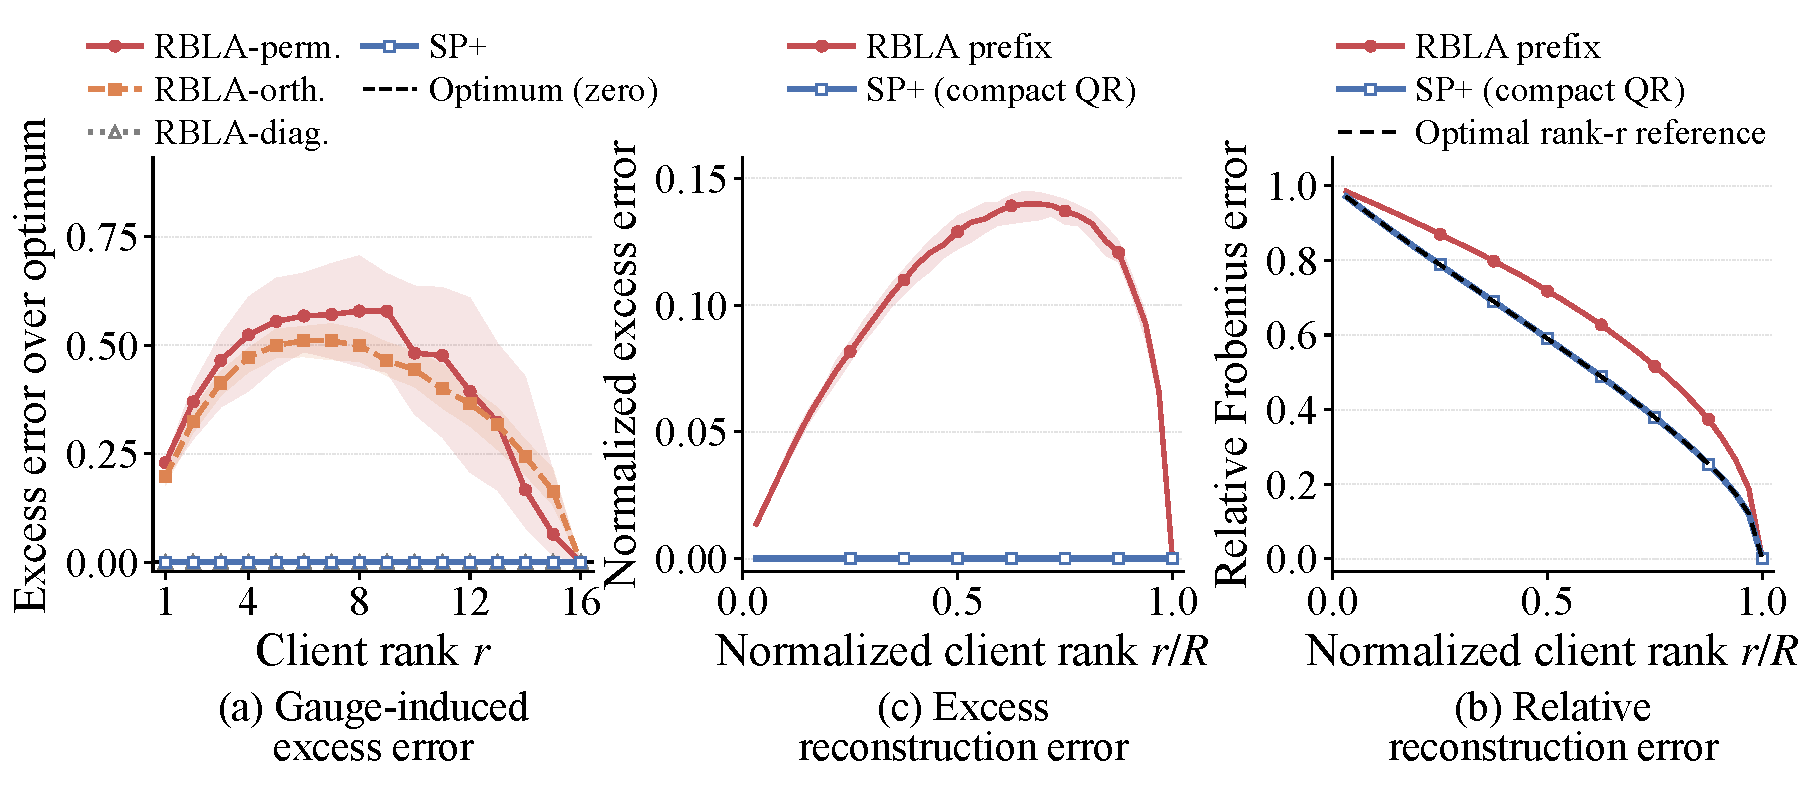
\includegraphics[width=\textwidth]{rbla+/figures/gauge_rbla_three_panel/gauge_rbla_three_panel.pdf}
  \caption{Gauge sensitivity and reconstruction error in synthetic RBLA aggregation.
  Panels are arranged from left to right as (a), (c), (b).
  (a) Gauge-induced excess error for a fixed $128\times96$ rank-16 update,
  using 100 trials per gauge type; diagonal scaling is a negative control.
  (b,c) Relative and normalized excess reconstruction errors in the synthetic
  RBLA aggregation experiment with 10 equally weighted clients, $512\times512$
  updates, $R=32$, client ranks $[8,8,12,12,16,16,20,24,28,32]$, and 30 fixed seeds.
  Shared Gaussian reference factors receive independent RMS-scaled perturbations
  with $\eta=0.3$. Each seed compares both methods on the same original RBLA
  aggregate with effective LoRA scaling one and no additional gauge transformation.
  Curves show pointwise medians and shaded bands indicate interquartile ranges.
  All errors use unsquared Frobenius norms; markers in (b,c) identify actual client ranks.
  The optimal reference overlaps the measured SP+ curve in (b).}
  \label{fig:gauge-rbla-reconstruction}
\end{figure*}
